\documentclass[dvipsnames]{beamer}
\usepackage[T1]{fontenc}
\usepackage{geometry}
\usepackage[utf8]{inputenc}
\usepackage{colortbl}
\usepackage[english]{babel}
\usepackage{pgf}
\usepackage{graphicx,epsfig, subfigure}
\usepackage{hyperref}
\usepackage{multirow}
\usepackage{minted}
\definecolor{lightgray}{rgb}{.3,.3,.3}
\usepackage{niceslides}

\title{Dependent Types \texttt{`mod`} Phase Distinction}

% Authors
\author{
  Joachim Tilsted Kristensen
}

% Affiliations
\institute{
  Univertity of Oslo
}

\date{Copenhagen, 22 Nov. 2022}

\begin{document}
\frame{\titlepage \vspace{-0.5cm}}

\begin{frame}{Propositions as types}
\end{frame}

\begin{frame}{Proofs as programs}
\end{frame}


\frame{
  \frametitle{Lambda Cube ($\lambda_\rightarrow$)}
  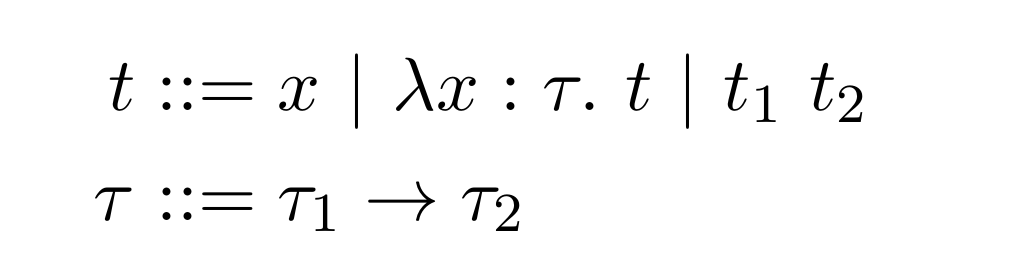
\includegraphics[width=0.5\textwidth]{./illustrations/lambda_calculus/basic_syntax}\\ \\

  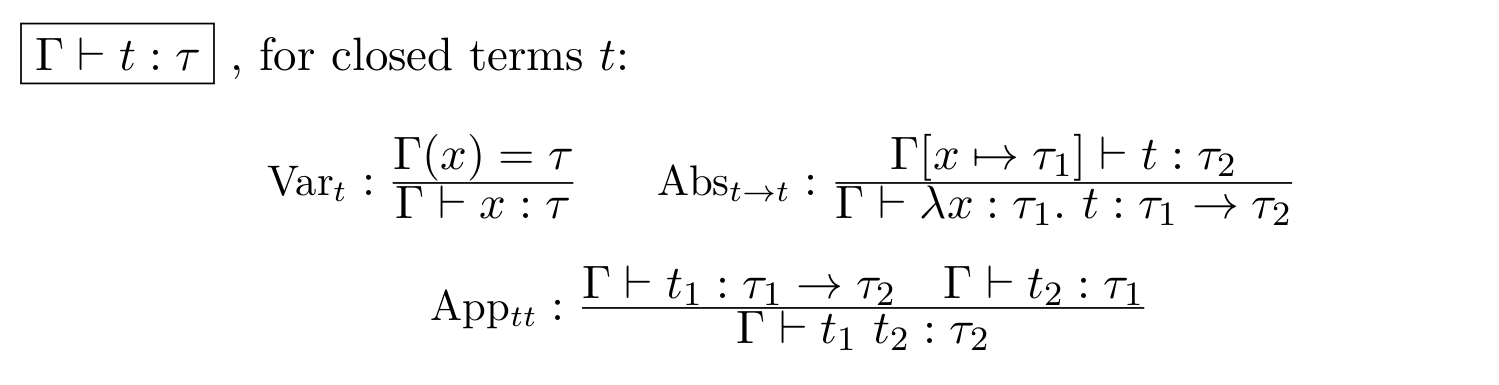
\includegraphics[width=\textwidth]{./illustrations/lambda_calculus/basic_typing}
}

\frame{
  \frametitle{Lambda Cube ($\lambda_2$)}
  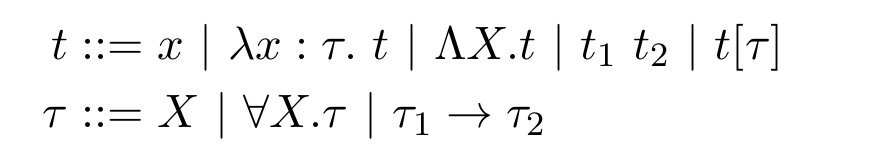
\includegraphics[width=0.5\textwidth]{./illustrations/lambda_calculus/polymorphic_syntax}\\
  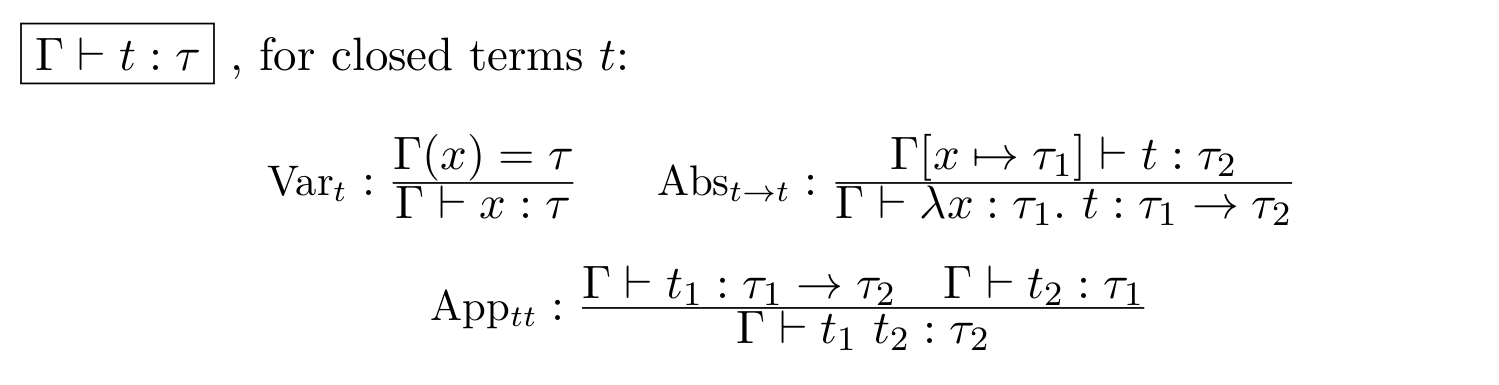
\includegraphics[width=\textwidth]{./illustrations/lambda_calculus/basic_typing}\\
  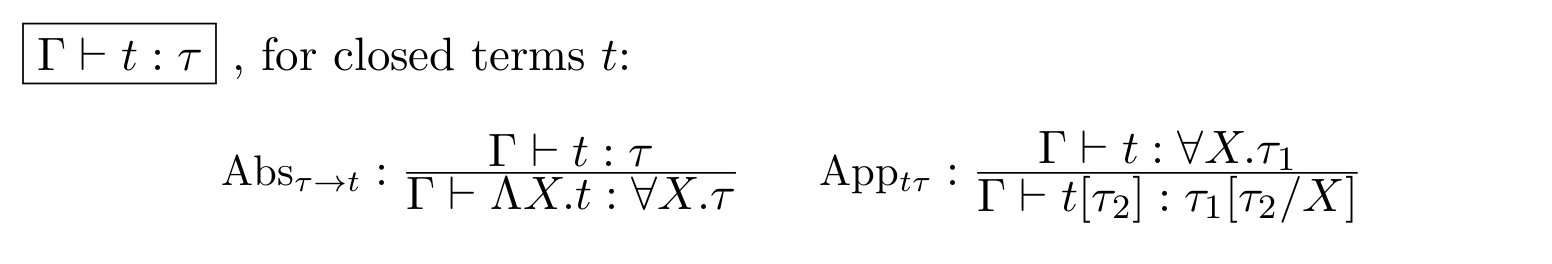
\includegraphics[width=\textwidth]{./illustrations/lambda_calculus/polymorphic_typing}
}

\frame{
  \frametitle{Lambda Cube ($\lambda_\omega$)}
  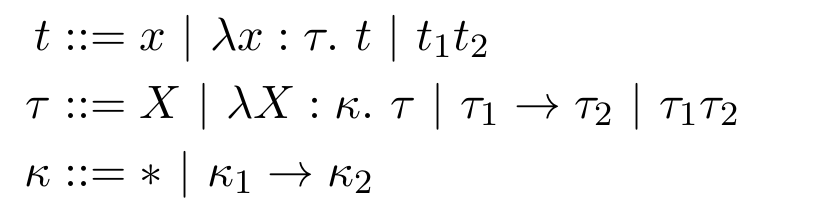
\includegraphics[width=0.5\textwidth]{./illustrations/lambda_calculus/type_level_syntax}\\
  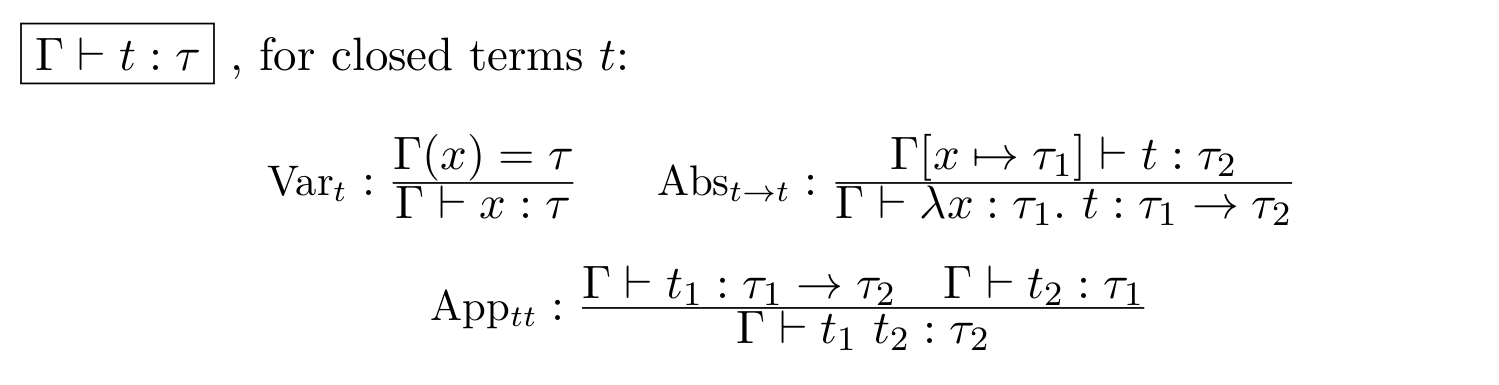
\includegraphics[width=\textwidth]{./illustrations/lambda_calculus/basic_typing}\\

  repeat Var$_t$, Abs$_{t\rightarrow{t}}$ and App$_{tt}$ to get Var$_\tau$, Abs$_{\tau\rightarrow\tau}$ and App$_{\tau\tau}$.
}

\frame{
  \frametitle{Lambda Cube ($\lambda_\Pi$)}
  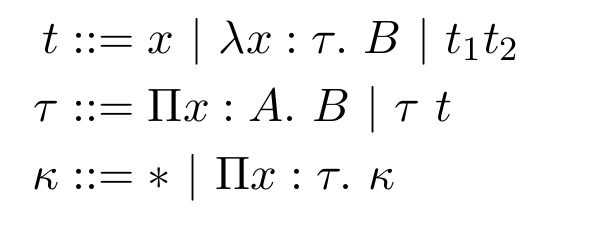
\includegraphics[width=0.5\textwidth]{./illustrations/lambda_calculus/dependent_syntax}\\
  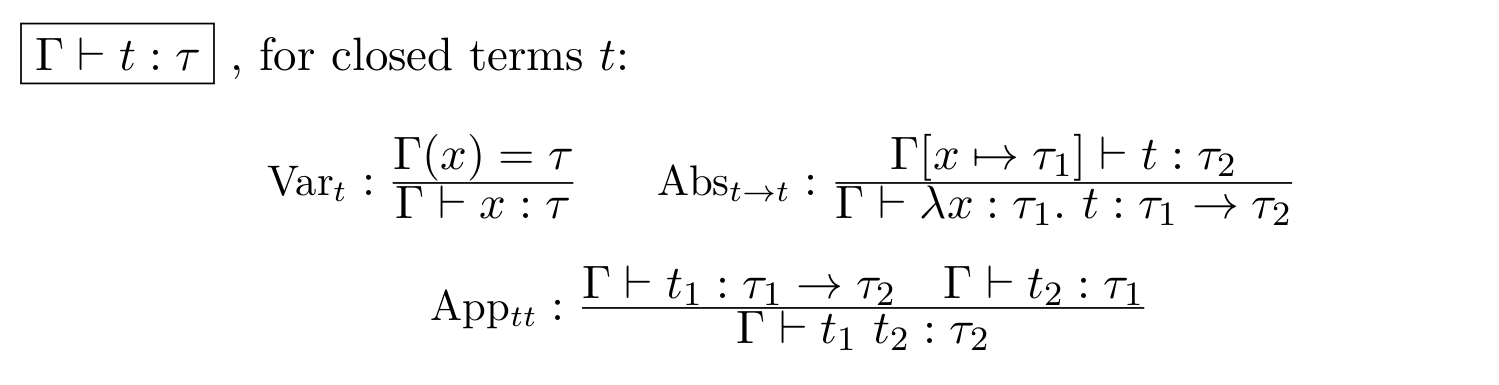
\includegraphics[width=0.9\textwidth]{./illustrations/lambda_calculus/basic_typing}\\
  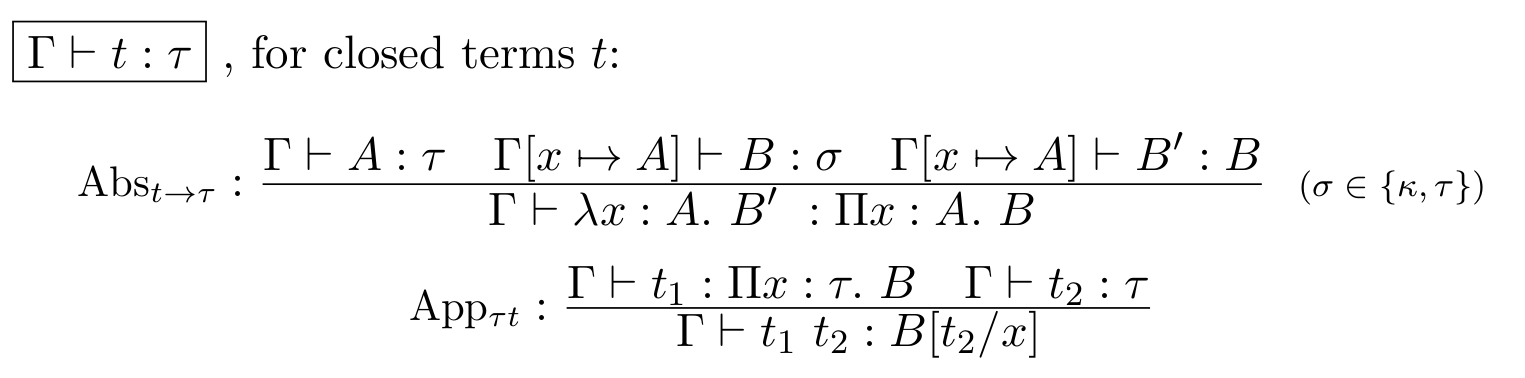
\includegraphics[width=0.9\textwidth]{./illustrations/lambda_calculus/dependent_typing}
}

\end{document}

%%% Local Variables:
%%% mode: latex
%%% TeX-master: t
%%% End:
